\chapter{Теоретичні відомості}


У цьому розділі буде розглянуто необхідний математичний апарат та теоретичні відомості стосовно проблеми яка лежить в основі даної магістерської дисертації. Розглянемо основне твердження теореми Шпернера та усі супутні визначення та твердження необхідні для вирішення поставленної задачі.


\section{Постановка задачі}
\newtheorem{shperner}{Теорема}
\begin{shperner}
Нехай $ M = \{1,...,n\} $ множина яка скаладється з елементів натурального ряду,
$M_1,...,M_k$ - підмножини множини $ M $ такі, що $ \forall M_i,M_j: M_i \not\subset M_j $, 
тоді виконується дуже проста нерівність $k \leq {C_n}^{[n/2]}$, де $ k $ - це кількість множин у наборі $M_1,...,M_k$, $ n $ - загальна кількість елементів множини $ M $ (тобто потужність множини $ M $, далі будемо позначати як $ |M| $), $ {C_n}^{[n/2]} $ - біноміальний коефіцієнт, $ [n/2] $ - ціла частина від діллення $ n $ навпіл. 
\end{shperner}


\\

Розглянемо одне з можливих доведь теореми базуючись на твердженні доведення якого буде представлене нижче.

\newtheorem{condition1}{Твердження}
\begin{condition1}
Нехай $ M_1,...,M_k $ - попарно невкладені одна в одну підмножини множини $ M = \{1,...,n\} $, нехай $ |M_1| = m_1,...,|M_k| = m_k $, тоді має місце нерівність:
\end{condition1}
\begin{large}
\begin{equation} \label{eq:binomial} 
\frac{1}{{C_n}^{m_1}} + \frac{1}{{C_n}^{m_2}} + ... + \frac{1}{{C_n}^{m_k}} \leq 1
\end{equation}
\end{large}
\newline


% Доведення Твердження 
\begin{proof}
Розглянемо для кожного $ M_i, i=1,..,k $ перестановки множини $ \{1,...,n\} $ зроблені по наступному принципу:

\begin{center}
\begin{tabular}{ |c|c|c|c|c|c|c|c|c|c|c| } 
 \hline
 $a_1$ & $a_2$ & . & . & $a_k$ & $a_{k+1}$ & . & . & . & . & $a_n$ \\
 \hline
\end{tabular}
\end{center}

Де $ a_1,...,a_k \in M_i $, а $ a_{k+1},...,a_n $ - всі інші елементи, тоді перша частина такої перестановки, тобто  $ a_1,...,a_k$ може мати $ (m_i)! $ різних варіантів, а права частина, тобто $ a_{k+1},...,a_n $, $ (n-m_i)!$ різних варіантів, де $n$ - потужність множини $ \{1,...,n\} $. Варто зазначити, що для різних множин $ M_i, M_j $ відповідні перестановки будуть відрізнятись. Якщо дві перестановки двох множин  $ M_i, M_j $ співпадають, це означає, що $ M_i \subseteq M_j $, або $ M_j \subseteq M_i $.
\\
Тому маємо:
\\
$m_1!(n-m_1)! + ... + m_k!(n-m_k)! \leq n! $, де $ n! $ - число усіх можливих перестановок множини $ \{1,...,n\} $. Розділимо обидві частини отриманої нерівності на $ n! $ та отримаємо суму обернених біноміальних коефіцієнтів з лівої частини та одиницю з правої: $\frac{1}{{C_n}^{m_1}} + \frac{1}{{C_n}^{m_2}} + ... + \frac{1}{{C_n}^{m_k}} \leq 1$, що і треба було довести.
\end{proof}

\newtheorem{corollary}{Наслідок}[condition1]
\begin{corollary}
Виходячи з формули (1.1) отримаємо, що кількість різних $ M_i $ не перевищує ${C_n}^{[n/2]}$. Так як ${C_n}^{m_i} \leq {C_n}^{[n/2]}$  маємо  $ \frac{1}{{C_n}^{[n/2]}} + \frac{1}{{C_n}^{[n/2]}} + ... + \frac{1}{{C_n}^{[n/2]}}   \leq \frac{1}{{C_n}^{m_1}} + \frac{1}{{C_n}^{m_2}} + ... + \frac{1}{{C_n}^{m_k}} \leq 1$, у найлівішій частині рівняння доданок $\frac{1}{{C_n}^{[n/2]}}$ зустрічається $k$ разів, тобто $\frac{k}{{C_n}^{[n/2]}} \leq 1$, або ж якщо записати у звичному вигляді $k \leq {C_n}^{[n/2]}$.
\end{corollary}

\par Поставлена задача узагальнити дану теорему на випадок коли множина $ M = \{1,...,n\} $ може мати кратні входження елементів, тобто математичний об'єкт $ M $ набуває мультимножинних властивостей. Дана задача вже була частково розглянута у бакалаврській дипломній роботі. Було розглянуто деякі часткові випадки мультимножин, які задовольняють умовам теореми. У даній роботі буде більш детально розглянуто прикладне застосування теореми, та узагальнення її на більшу кількість окремих випадків мультимножин. Для того, щоб математичні викладки та послідовність дій була зрозумілою унаступному розділі наводяться необхідні теоретичні відомості та означення базуючись на яких було отримано результати, які будуть описані нижче.

\section{Теорія мультимножин}




\newpage

\section{Постановка задачі}


\\

\begin{center}
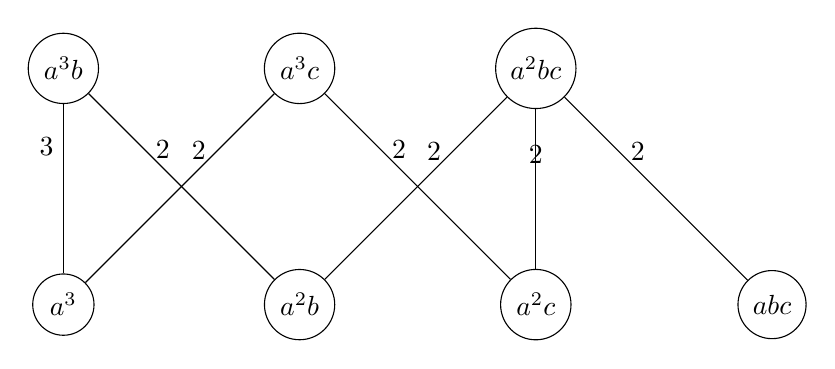
\begin{tikzpicture}[node distance={30mm}, main/.style = {draw, circle}] 
\node[main] (1) {$a^3b$}; 
\node[main] (2) [right of=1] {$a^3c$}; 
\node[main] (3) [right of=2] {$a^2bc$}; 
\node[main] (4) [below of=1] {$a^3$}; 
\node[main] (5) [below of=2] {$a^2b$}; 
\node[main] (6) [below of=3] {$a^2c$}; 
\node[main] (7) [right of=6] {$abc$}; 

\draw (1) -- node[pos=0.25, left] {3} (4); 
\draw (1) -- node[pos=0.4, above] {2} (5); 
\draw (2) -- node[pos=0.4, above] {2}(4); 
\draw (2) -- node[pos=0.4, above] {2}(6); 
\draw (3) -- node[pos=0.4, above] {2}(5); 
\draw (3) -- node[pos=0.4, above] {2}(6); 
\draw (3) -- node[pos=0.4, above] {2}(7); 
\end{tikzpicture} 
\end{center}
\newpage


\subsection{Попередні роботи} 
\subsection{Визначення}
\section{Розв'язок}
